% Derived From ACM's "SIGPROC-SP.TEX - VERSION 3.1"

\documentclass{acm_proc_article-sp}
\usepackage{color, soul}
\newcommand{\Comment}[2]{{\color{red}{#1} :::  \color{blue}{#2}}\\}

\begin{document}

\title{Beautiful Scalable Awesome Interpretable CX Matrix Factorization for Bio-Imaging}
%
% You need the command \numberofauthors to handle the 'placement
% and alignment' of the authors beneath the title.
%
% For aesthetic reasons, we recommend 'three authors at a time'
% i.e. three 'name/affiliation blocks' be placed beneath the title.
%
% NOTE: You are NOT restricted in how many 'rows' of
% "name/affiliations" may appear. We just ask that you restrict
% the number of 'columns' to three.
%
% Because of the available 'opening page real-estate'
% we ask you to refrain from putting more than six authors
% (two rows with three columns) beneath the article title.
% More than six makes the first-page appear very cluttered indeed.
%
% Use the \alignauthor commands to handle the names
% and affiliations for an 'aesthetic maximum' of six authors.
% Add names, affiliations, addresses for
% the seventh etc. author(s) as the argument for the
% \additionalauthors command.
% These 'additional authors' will be output/set for you
% without further effort on your part as the last section in
% the body of your article BEFORE References or any Appendices.

\numberofauthors{8} %  in this sample file, there are a *total*
% of EIGHT authors. SIX appear on the 'first-page' (for formatting
% reasons) and the remaining two appear in the \additionalauthors section.
%
\author{
% You can go ahead and credit any number of authors here,
% e.g. one 'row of three' or two rows (consisting of one row of three
% and a second row of one, two or three).
%
% The command \alignauthor (no curly braces needed) should
% precede each author name, affiliation/snail-mail address and
% e-mail address. Additionally, tag each line of
% affiliation/address with \affaddr, and tag the
% e-mail address with \email.
%
% 1st. author
\alignauthor
Ben Trovato\titlenote{Dr.~Trovato insisted his name be first.}\\
       \affaddr{Institute for Clarity in Documentation}\\
       \affaddr{1932 Wallamaloo Lane}\\
       \affaddr{Wallamaloo, New Zealand}\\
       \email{trovato@corporation.com}
% 2nd. author
\alignauthor
G.K.M. Tobin\titlenote{The secretary disavows
any knowledge of this author's actions.}\\
       \affaddr{Institute for Clarity in Documentation}\\
       \affaddr{P.O. Box 1212}\\
       \affaddr{Dublin, Ohio 43017-6221}\\
       \email{webmaster@marysville-ohio.com}
% 3rd. author
\alignauthor Lars Th{\o}rv{\"a}ld\titlenote{This author is the
one who did all the really hard work.}\\
       \affaddr{The Th{\o}rv{\"a}ld Group}\\
       \affaddr{1 Th{\o}rv{\"a}ld Circle}\\
       \affaddr{Hekla, Iceland}\\
       \email{larst@affiliation.org}
\and  % use '\and' if you need 'another row' of author names
% 4th. author
\alignauthor Lawrence P. Leipuner\\
       \affaddr{Brookhaven Laboratories}\\
       \affaddr{Brookhaven National Lab}\\
       \affaddr{P.O. Box 5000}\\
       \email{lleipuner@researchlabs.org}
% 5th. author
\alignauthor Sean Fogarty\\
       \affaddr{NASA Ames Research Center}\\
       \affaddr{Moffett Field}\\
       \affaddr{California 94035}\\
       \email{fogartys@amesres.org}
% 6th. author
\alignauthor Charles Palmer\\
       \affaddr{Palmer Research Laboratories}\\
       \affaddr{8600 Datapoint Drive}\\
       \affaddr{San Antonio, Texas 78229}\\
       \email{cpalmer@prl.com}
}
% There's nothing stopping you putting the seventh, eighth, etc.
% author on the opening page (as the 'third row') but we ask,
% for aesthetic reasons that you place these 'additional authors'
% in the \additional authors block, viz.
\additionalauthors{Additional authors: John Smith (The Th{\o}rv{\"a}ld Group,
email: {\texttt{jsmith@affiliation.org}}) and Julius P.~Kumquat
(The Kumquat Consortium, email: {\texttt{jpkumquat@consortium.net}}).}
\date{30 July 1999}
% Just remember to make sure that the TOTAL number of authors
% is the number that will appear on the first page PLUS the
% number that will appear in the \additionalauthors section.

\maketitle
\begin{abstract}
We investigate the performance, scalability, and applicability of low-rank matrix approximation algorithms, including randomized PCA and randomized CX/CUR low-rank matrix factorizations, on a 1 TB mass spectrometry imaging (MSI) dataset, using Apache Spark on an Amazon EC2 cluster, a 
Cray~XC40 system, and an experimental Cray cluster.
While these low-rank matrix computations are popular in small- to medium-scale machine learning and scientific data analysis, computing them provides a much more powerful ``stress test'' of linear algebra algorithms in large-scale distributed analytics frameworks than is provided by, e.g., low-precision PageRank computations.
In addition, scientific applications such as MSI data analysis provides a very different use case 
than is provided by typical commercial workloads.
We implemented these algorithms in Scala using the Apache Spark high-level cluster computing framework.  
We obtained competitive performance on all three platforms; we were able to process the 1TB size dataset in under 30 minutes with 960 cores on all systems, with the fastest times obtained on the experimental Cray cluster.
We report these results, and conclude broader implications for hardware and software issues for supporting data-centric workloads in parallel and distributed environments.  

\end{abstract}

% A category with the (minimum) three required fields
\category{H.4}{Information Systems Applications}{Miscellaneous}
%A category including the fourth, optional field follows...
\category{D.2.8}{Software Engineering}{Metrics}[complexity measures, performance measures]

\terms{Theory}

\keywords{ACM proceedings, \LaTeX, text tagging} % NOT required for Proceedings

\section{Introduction}
\label{sec:intro}

Matrix algorithms are increasingly important in many large-scale data analysis applications.
Essentially, the reason is that matrices (i.e., sets of vectors in Euclidean
spaces) provide a convenient mathematical structure with which to model data
arising in a broad range of applications

In particular, the low-rank approximation to a data matrix $A$ that is provided
by performing a truncated SVD (singular value decomposition)---or PCA
(principal component analysis) or CX/CUR decompositions---is a very complicated
object compared with what is conveniently supported by traditional database
operations~\cite{Skillicorn07}. Recall that PCA finds mutually orthogonal
directions that maximize the variance captured by the factorization, and CX/CUR
provides an interpretable low-rank factorization by selecting a small number of
columns/rows from the original data matrix.  Described in more detail in
Section~\ref{sxn:low-rank-methods}, these low-rank approximation methods are
popular in small- and medium-scale machine learning and scientific data
analysis applications for exploratory data analysis and for
providing compact and interpretable representations of complex matrix-based
data, but their implementation at scale remains a challenge.

These matrix-based methods do not mesh well with much of the work that has been popular recently in large scale data analysis.
For example, MapReduce/Hadoop does a certain amount of reading and writing at every step and thus iterative algorithms are prohibitive~\cite{DG08_CACM}.
Apache Spark solves some of these problems by maintaining additional state, but even there systems are not designed for nontrivial matrix algorithms~\cite{SPARK_NSDI_12}. There is an associated question of the ideal hardware platform for running Big Data Analytics. Conventional EC2 class hardware utilizes loosely coupled nodes; whereas typical HPC system are much more tightly coupled with high performance interconnects. Frameworks such as Hadoop and Spark have been developed for EC2 class hardware, and their performance on HPC hardware, especially for complex analytics problems (including matrix decompositions) is largely unexplored. 

In this paper, we address the following research questions:
\begin{itemize}
\item Can we successfully apply low rank matrix factorization methods (such as CX) to a TB-scale scientific dataset?

\item Can we implement CX in a contemporary data analytics framework such as Spark?

\item What is the performance gap between a highly tuned C, and a Spark-based CX implementation? 

\item How well does a Spark-based CX implementation scale on modern HPC and data-center hardware platforms?
\end{itemize}

We start with a description of matrix factorization algorithms in Section~\ref{sxn:low-rank-methods}, followed by single node and multi-node implementation details in Section~\ref{sec:implementation}. We review the experimental setup for our performance tests in Section~\ref{sec:setup}, followed by results and discussion in Section~\ref{sec:results}.


\section{Low-rank matrix factorization methods}
\label{sxn:low-rank-methods}
%% \textit{Owners: Jiyan, Michael Mahoney (1 page)}

Given an $m \times n$ data matrix $A$, low-rank matrix factorization methods aim to find two or more smaller matrices such that their product is a good approximation to $A$.
That is, they aim to find matrices $Y$ and $Z$ such that
\begin{equation}
 \label{eqn:apprx}
    \underset{m\times n}{A} \approx \underset{m\times k}{Y} \times \underset{k\times n}{Z} , 
\end{equation}
where $Y \times Z$ is a rank-$k$ approximation to the original matrix $A$.
Low-rank matrix factorization methods are an important topic in linear algebra and numerical analysis, and they find use in a variety of scientific fields and scientific computing as well as in machine learning and data analysis applications such as pattern recognition and personalized recommendation.

Depending on the application, various low-rank factorization techniques are of interest. 
Popular choices include the singular value decomposition~\cite{GVL96}, principal component analysis~\cite{pcaBook}, rank-revealing QR factorization~\cite{GE96}, nonnegative matrix factorization~\cite{NMFalg}, and CUR/CX decompositions~\cite{CUR_PNAS}.
In this work, we consider using the SVD and CX decompositions for our scalable and interpretable data analysis; and, in the remainder of the section, we briefly describe these decompositions.
For an arbitrary matrix $A$, denote by $\a_i$ its $i$-th row, $\a^j$ its $j$-th column and $\a_{ij}$ its $(i,j)$-th element. 
Hereby, we assume the data matrix $A$ has size $m \times n$ and rank $r$.


\subsection{SVD and PCA}

The singular value decomposition (SVD) is the factorization of matrix $A \in \reals^{m\times n}$ into the product of three matrices $U\Sigma V^T$ where $U \in \reals^{m\times r}$ and $V\in \reals^{n\times r}$ have orthonormal columns and $\Sigma\in \reals^{r\times r}$ is a diagonal matrix with positive real entries. 
The columns of $U$ and $V$ are called left and right singular vectors and the diagonal entries of $\Sigma$ are called singular values. 
For notation convenience, we assume the singular values are sorted such that $\sigma_1\geq \cdots \geq \sigma_r\geq 0$, and this means that the columns of $U$ and $V$ are sorted by the order given by the singular values.  

%if optimality criterion to choose is the square loss ($\ell_2$ loss)
 
The SVD is of central interest because it provides the ``best'' low-rank matrix approximation with respect to any unitarily invariant matrix norm.
In particular, for any target rank $k \leq r$, the SVD provides the minimizer of the optimization problem
\begin{equation}
 \label{eqn:obj}
  \min_{\text{rank}(\tilde A) = k} \| A - \tilde A \|_F,
\end{equation}
where the Frobenius norm $\| \cdot \|_F$ is defined as $\|X\|_F^2 =
\sum_{i=1}^m \sum_{j=1}^n X_{ij}^2 $. Specifically, the solution
to~\eqref{eqn:obj} is given by the truncated SVD, i.e., $A_k = U_k \Sigma_k
V_k^T$, where the columns of $U_k$ and $V_k$ are the top $k$ singular vectors,
i.e., the first $k$ columns of $U$ and $V$, respectively, and $\Sigma_k$ is a 
diagonal matrix containing the top-$k$ singular values.

Principal component analysis (PCA) and SVD are closely related.
PCA aims to convert the original features into a set of linearly uncorrelated variables called {\it principal components}.
To be more specific, the first principal component is defined to be the direction along which the highest variance possible among the data points is attained, and each succeeding principal component in turn has the largest variance possible subject to the constraint that it is orthogonal to the preceding principal components.
When low-rank methods are appropriate, the number of principal components needed to preserve most of the information in $A$ is far less than the number of original features, and thus the goal of dimension reduction is achieved.
The PCA decomposition of $A$ is defined as the SVD of the matrix formed by centering each column of $A$ (i.e., removing the mean of each column).

\subsection{Randomized SVD}

The computation of the SVD (and thus of PCA for a data matrix $A$) is
expensive~\cite{GVL96}.  For example, to compute the truncated SVD with rank
$k$ using traditional deterministic methods, the running time complexity is
$\bigO(mnk)$, and $\bigO(k)$ passes over the dataset are needed.  This  becomes
prohibitively expensive when dealing with datasets of even moderately-large
size, e.g., $m = 10^6$, $n = 10^4$ and $k = 20$.  To address these and related
issues, recent work in Randomized Linear Algebra (RLA) has focused on using
randomized approximation, e.g., random projection and random sampling methods,
to perform scalable linear algebra computations\footnote{For example, RLA
  algorithms have led to the best worst-case algorithms for least squares and
  least absolute deviations regression, they have been implemented to high
  precision and have been shown to beat LAPACK's direct dense least squares
  solver on essentially any tall dense matrix; they have been been shown to
  lead to improved low-rank matrix approximation in scientific computing
  applications, and they have been shown to have improved statistical
  properties~\cite{Mah-mat-rev_BOOK}.  Thus, while our focus here is on
  improved low-rank matrix approximation methods in Spark, we expect that
  similar improvements can be achieved for other related problems.} for
large-scale data problems.  For an overview of the RLA area,
see~\cite{Mah-mat-rev_BOOK}; for a review of using RLA methods for low-rank
matrix approximation, see~\cite{HMT09_SIREV}; and for a review of the theory
underlying implementing RLA methods in parallel/distributed environments,
see~\cite{YMM15_TR}.

Here, we will use an algorithm described in Halko et al.~\cite{HMT09_SIREV}
which uses a random projection to construct a rank-$k$ approximation to $A$
which approximates $A$ nearly as well as $A_k$ does.  We refer the readers to
\cite{HMT09_SIREV,Mah-mat-rev_BOOK} for more details.  Importantly, the
algorithm runs in $\bigO(mn \log k)$ time, and the algorithm needs only a
constant number of passes over the data matrix.  These properties becomes
extremely desirable in many large-scale data analytics.  This algorithm, which
we refer to as \textsc{RandomizedSVD}, is summarized in
Algorithm~\ref{alg:rsvd}.  (Algorithm~\ref{alg:rsvd} calls
\textsc{MultiplyGramian}, which is summarized in Algorithm~\ref{alg:gram}, as
well as three algorithms, \textsc{Multiply}, \textsc{ThinQR}, and
\textsc{ThinSVD}, which are standard in numerical linear algebra~\cite{GVL96}.)
The running time cost for \textsc{RandomizedSVD} is dominated by the
matrix-matrix multiplication, which involve passing over the entire data
matrix, appearing in Step 3 and Step 7 of Algorithm~\ref{alg:rsvd}.  
These steps can be parallelized, and hence \textsc{RandomizedSVD} is well
amenable to distributed computing.
% \footnote{We should mention that Step 3 of
%Algorithm~\ref{alg:rsvd} involves a dense matrix-matrix multiplication, whereas
%most RLA algorithms, including the variant of \textsc{RandomizedSVD}
%in~\cite{HMT09_SIREV} uses an FFT-based random projection in order to obtain a
%faster asymptotic running time.  While our version incurs more FLOPS, it is
%more parallelizable and thus more suitable for distributed computational
%environments.}


\begin{algorithm}[tb]
 \caption{{\sc RandomizedSVD} Algorithm}
  \label{alg:rsvd}
  \begin{algorithmic}[1]
    \Require $A \in \reals^{m\times n}$, \
      number of power iterations $q \ge 1$, \
      target rank $r > 0$, slack $\ell \ge 0$, and let $k=r+\ell$.

    % TODO: domain of each result
    \Ensure $U \Sigma V^T \approx \Call{ThinSVD}{A, r}$.

    \State Initialize $B \in \reals^{n\times k}$ by sampling $B_{ij} \sim \mathcal{N}(0, 1)$.

    \For{$q$ times}
        \State $B \gets \Call{MultiplyGramian}{A, B}$
        \State $(B, \_) \gets \Call{ThinQR}{B}$
    \EndFor

    \State Let $Q$ be the first $r$ columns of $B$.

    \State Let $C = \Call{Multiply}{A, Q}$.

    \State Compute $(U, \Sigma, \tilde V^T) = \Call{ThinSVD}{C}$.

    \State Let $V = Q \tilde V$.
    % alternative that doesn't require knowing the distributivity of transpose but looks silly:
    %\State Let $V^T = \tilde V^T Q^T$.

    \end{algorithmic}
\end{algorithm}

\begin{algorithm}[tb]
  \caption{{\sc MultiplyGramian} Algorithm}
  \label{alg:gram}
  \begin{algorithmic}[1]
    \Require $A \in \reals^{m\times n}$, $B \in \reals^{n\times k}$.
    \Ensure $X = A^T A B$.
    \State Initialize $X = 0$.
    \For{each row $a$ in $A$}
        \State $X \gets X + a a^T B$.
    \EndFor
  \end{algorithmic}
\end{algorithm}


\subsection{CX/CUR decompositions}

In addition to developing improved algorithms for PCA/SVD and related problems,
work in RLA has also focused on so-called CX/CUR
decompositions~\cite{DMM08,CUR_PNAS}.  As a motivation, observe that singular
vectors are eigenvectors of the Gram matrix $A^TA$, and thus they are linear
combinations of up to all of the original variables.  A natural question
arises: can we reconstruct the matrix using a small number of actual columns of
$A$?

CX/CUR decompositions affirmatively answer this question.  That is, these are
low-rank matrix decompositions that are expressed in terms of a small number of
columns/rows, i.e, actual data elements, and not a small number of
eigencolumns/eigenrows (which form the principal components).  As such, they
have found applicability in scientific applications where coupling analytical
techniques with domain knowledge is at a premium, including
genetics~\cite{Paschou07b}, astronomy~\cite{Yip14-AJ}, and mass spectrometry
imaging~\cite{YRPMB15}.

In more detail, CX decomposition factorizes an $m \times n$ matrix $A$ into two
matrices $C$ and $X$, where $C$ is an $m\times c$ matrix that consists of $c$
actual columns of $A$, and $X$ is a $c \times n$ matrix such that $A\approx
CX$.
%That is, linear combinations of the columns of $C$ can recover most of the
%``information'' of the matrix $A$.
(CUR decompositions further choose $X=UR$, where $R$ is a small number of actual rows
of $A$~\cite{DMM08,CUR_PNAS}.)
For CX, using the same optimality criterion defined in~\eqref{eqn:obj}, we seek
matrices $C$ and $X$ such that the residual error $\|A-CX\|_F$ is small.

The algorithm of~\cite{DMM08} that computes a $1\pm\epsilon$ relative-error
low-rank CX matrix approximation consists of three basic steps: first, compute
(exactly or approximately) the {\it statistical leverage scores} of the columns
of $A$; and second, use those scores as a sampling distribution to select $c$
columns from $A$ and form $C$; finally once the matrix $C$ is determined, the
optimal matrix $X$ with rank-$k$ that minimizes $\|A-CX\|_F$ can be computed
accordingly; see~\cite{DMM08} for detailed construction. In this paper we focus
on the first two steps.  

\begin{algorithm}[tb]
 \caption{\textsc{CXDecomposition}}
  \label{alg:cx}
  \begin{algorithmic}[1]
    \Require $A \in \reals^{m\times n}$, rank parameter $k \leq \textrm{rank}(A)$, number of power iterations $q$.

    \Ensure $C$.
    
    %\Function{ColSelect}{$A,k,r$}

    %\State Using algorithm of\cite{DMMW12_JMLR}, compute an approximation of the top-$k$ right singular vectors of $A$ denoted by $\tilde V_k$, using \textsc{RandomizedSVD} with $q$ power iterations.
    \State Compute an approximation of the top-$k$ right singular vectors of $A$ denoted by $\tilde V_k$, using \textsc{RandomizedSVD} with $q$ power iterations.
    
    \State Let $\ell_i = \sum_{j=1}^k \tilde \v_{ij}^2$, where $\tilde \v_{ij}^2$ is the $(i,j)$-th element of $\tilde V_k$, for $i = 1, \ldots, n$. 
    
    \State Define $p_i = \ell_i / \sum_{j=1}^d \ell_j$ for $i=1,\ldots,n$.
    
    \State Randomly sample $c$ columns from $A$ in i.i.d. trials, using the importance sampling distribution $\{p_i\}_{i=1}^n$ .

    %\State \Return The indices with the top $r$ $\ell_i$s.
    
    %\EndFunction

    \end{algorithmic}
\end{algorithm}

The algorithm for approximating the leverage scores is
provided in Algorithm~\ref{alg:cx}.
Let $A=U\Sigma V^T$ be the SVD of $A$.
Given a target rank parameter $k$, for $i=1,\ldots,n$, the $i$-th leverage score is defined as
\begin{equation}
 \label{eqn:lev}
  \ell_i = \sum_{j=1}^k \v_{ij}^2.
\end{equation}
These scores quantify the amount of ``leverage'' each column of $A$ exerts on the best rank-$k$ approximation to $A$. 
For each column of $A$, we have 
  $$  \a_i = \sum_{j=1}^{r} (\sigma_j \u_j) \v_{ij} \approx \sum_{j=1}^k (\sigma_j \u_j) \v_{ij}.  $$
  That is, the $i$-th column of $A$ can be expressed as a linear combination of the basis of the dominant $k$-dimensional left singular space with $\v_{ij}$ as the coefficients.
If, for $i=1,\ldots,n$, we define the {\it normalized leverage scores} as
\begin{equation}
\label{eqn:nlev}
  p_i = \frac{\ell_i}{\sum_{j=1}^n \ell_j},
\end{equation}      
where $\ell_i$ is defined in~\eqref{eqn:lev}, and choose columns from $A$ according to those normalized leverage scores, then (by~\cite{DMM08,CUR_PNAS}) the selected columns are able to reconstruct the matrix $A$ nearly as well as $A_k$ does.

Observe that the running time for \textsc{CXdecomposition} is determined by the computation of the importance sampling distribution.
To compute the leverage scores based on \eqref{eqn:lev}, i.e., exactly, one needs to compute the top $k$ right-singular vectors $V_k$. 
As pointed out above, this is prohibitive data with massive size.
However, just as with our SVD computation, here we can use \textsc{RandomizedSVD} to compute {\it approximate} leverage scores.
This approach, originally proposed by Drineas et al.~\cite{DMMW12_JMLR}, runs in ``random projection time,'' i.e., it requires fewer FLOPS and fewer passes over the data matrix than the traditional deterministic algorithms that compute the leverage scores~exactly.


%Finally, we want to point out that,
%although delivering different low-rank factorizations, both PAC and CX suffer from the fact that they need to truncated SVD.
%To make the algorithms practical on large-scale dataset, one can alleviate the demanding complexity by using randomized SVD. 

%These algorithms compute high-quality approximations to the normalized leverage scores of the input matrix, and the running time of these algorithms depends on the time to apply a random projection to the input matrix, which is much faster than computing the full (or even a truncated) SVD.


\begin{figure*}[htp]
\includegraphics[scale=0.254]{images/jatin_a}
\includegraphics[scale=0.254]{images/jatin_b}
\caption{ Data access pattern for computing ${C}_{\it{i}}$ (left) and {\it{Res}}$_{\it{j}}$ (right) respectively.}
\label{fig:access_pattern}
\end{figure*}

\section{High Performance Implementation}
\label{sec:implementation}

We undertake two classes of high performance implementations for the CX method. 
We start with a highly optimized, close-to-the-metal C implementation
that focuses on obtaining peak efficiency from conventional multi-core
CPU chipsets and extend it to multiple nodes. 
%%%The purpose of this exercise is to establish a baseline for the CX method. 
Secondly, we implement the CX method in Spark, an emerging standard for parallel data analytics frameworks. 
%%%%%%%%%%%%%%%%%%%%%Implementing the method in Spark provides us with a scalable strategy to run on multiple nodes, and tackle a large scale dataset. 



\subsection {Single Node Implementation/Optimizations}
\label{sxn:single_node_opt}

    We now focus on optimizing the CX implementation on a single
    compute-node.
    %, aimed at exploiting the available SIMD units on each core, and the multiple cores across different sockets to speed up the performance. 
    We began by profiling our initial %%unoptimized 
    scalar serial CX
    code and optimizing the steps in the order of execution times.
    The most time is spent in computing sparse-sparse-dense matrix
    multiplication ($A^TAB$, Step 3, 90.6\%), followed by  sparse-dense matrix
    multiplication ($AQ$, Step 7, 9.1\%) and finally, QR
    decomposition (Step 4, 0.4\%)
    for a representative dataset that fits in main memory. These
    three kernels account for more than 99.9\% of
    the execution time.
    Recall that $A$ is a sparse matrix with dimensions
    $m \times n$
    and sparsity $s$, and $B$ is a dense $n \times k$ matrix.
    %%We first discuss the case of $A^TAB$.

\vspace*{0.05in} 
\subsubsection{Optimizing $\mathrm{Res}=A^TAB$}
    Optimizing sparse matrix-matrix  multiplication continues to be an
    active area of research~\cite{ballard13,patwary15}, with focus on
    reducing communication, and the state of the art implementations
    are bound by the memory bandwidth and heavily
    underutilize the compute resources. 
    %%
    %%As far as computing $A^TAB$ is concerned, 
    For our application, we exploit the following three observations:
    (1) One of the sparse matrices is the transpose of the other,   
    (2) One of the matrices is a dense matrix,   and    %%The sparse-sparse matrix multiplication is followed by a sparse-dense matrix multiplication. 
    (3) $n \gg k$ and $sm \gg k$.

    Exploiting associativity of multiplication, we perform $C$ = $AB$, 
    followed by $\mathrm{Res} = A^TC$. This reduces the run-time complexity from
    O({\it{n*(nsm)}}) to O({\it{k*(nsm)}}). Furthermore, we do not
    explicitly compute (or store) the transpose of $A$.  Consider the
    ${\it{i}}^{th}$ row, $A_i$. 
    By definition,  $C_i = A_i \cdot B$.
    The (${\it{j}},{\it{l}}$)$^{th}$ element of $\mathrm{Res}$,
    $\mathrm{Res}_{{\it{j}},{\it{l}}}$ =
    $\Sigma_{\it{p}}$($A^T_{{\it{j}},{\it{p}}}$ x $C$$_{{\it{p}},{\it{l}}}$) = 
    $\Sigma_{\it{p}}$($A_{{\it{p}},{\it{j}}}$ x
    $C$$_{{\it{p}},{\it{l}}}$).
%% 
%% 
%% 
%% 
    For {\it{p}} = {\it{i}}, this reduces to incrementing
    $\mathrm{Res}_{{\it{j}},{\it{l}}}$ by $A_{{\it{i}},{\it{j}}}$ x
    $C$$_{{\it{i}},{\it{l}}}$. 
%% 
%% 
%% 
    Thus, for each row {\it{i}}, 
    %having computed C$_{\it{i}}$, we can scale each entry by  $A_{{\it{i}},{\it{j}}}$ 
    having computed C$_{\it{i}}$, we
    increment $\mathrm{Res}_{{\it{j}},{\it{l}}}$ 
    by $A_{{\it{i}},{\it{j}}}$ x $C$$_{{\it{i}},{\it{l}}}$
    for {\it{j}}$\in$[1..{\it{n}}] and {\it{l}}$\in$[1..{\it{k}}].
     We now describe how we parallelize  to exploit
     data- and thread-level parallelism and other relevant
     optimizations.

     %%%%%%%%%%%%%%%%%%%%%%%%%%%%%%%%%%%%%%%%%%%%%%%%%%%%%%%%%%%%%%%%%%%%%%%%%%%%%%%%%%%%%%%%%%%%%%%%%%%%%%%%%%%%%%%%%%%%%




     %%%%%%%%%%%%%%%%%%%%%%%%%%%%%%%%%%%%%%%%%%%%%%%%%%%%%%%%%%%%%%%%%%%%%%%%%%%%%%%%%%%%%%%%%%%%%%%%%%%%%%%%%%%%%%%%%%%%%
     %%%%%%%%%%%%%%%%%%%%%%%%%%%%%%%%%%%%%%%%%%%%%%%%%%%%%%%%%%%%%%%%%%%%%%%%%%%%%%%%%%%%%%%%%%%%%%%%%%%%%%%%%%%%%%%%%%%%%
     \vspace*{0.05in}
     {\it{1. Exploiting SIMD}}: Refer to Figure~\ref{fig:access_pattern}. 
     Consider element $A_{{\it{i}},{\it{j}}}$. To compute
     $C_{\it{i}}$, we need to scale each element of
     $B_{{\it{j}}}$ by  $A_{{\it{i}},{\it{j}}}$ and add it to
     $C_{\it{i}}$ ({\it{j}}$\in$[1..{\it{n}}]) ($C_{\it{i}}$ +=
     $A_{{\it{i}},{\it{j}}}$ x $B_{{\it{j}}}$). Note that there are
     {\it{k}} elements in $B_{{\it{j}}}$, which are also stored
     consecutively (matrix stored in a row-major fashion).
%%
     On modern computing platforms, SIMD width (number of simultaneous
     operations that can be performed) is
     growing~\cite{intel2}. SSE can perform 4
     single-precision floating point computations in a single op, while
     AVX %%(our SPARK platform) 
     performs 8 ops. Let $\mathcal{S}$ denote the SIMD width
     (defined as number of double-precision floating point ops. per op
     -- which is half of single-precision ops).
    %% 
     The pseudo-code~\footnote{Exact syntax varies with the ISA and
     compiler version.} for computing $C_{\it{i}}$ ($\forall$
     $A_{{\it{i}},{\it{j}}}$ $\neq$ 0):
     \vspace*{0.03in}

     \hspace*{-0.13in}xmm\_a = {\it{vec\_load\_and\_splat}}($A_{{\it{i}},{\it{j}}}$); \\
     for\hspace*{0.02in}({\it{z}} = 0; {\it{z}} $<$ {\it{k}}; {\it{z}} += $\mathcal{S}$)\\
     \{\\
         \hspace*{0.2in}xmm\_c = {\it{vec\_load}}  ($C_{{\it{j}}}$ + z); \\
         \hspace*{0.2in}xmm\_b = {\it{vec\_load}}  ($B_{{\it{j}}}$ + z); \\
         \hspace*{0.2in}xmm\_ab = {\it{vec\_mul}}  (xmm\_a, xmm\_b); \\
         \hspace*{0.2in}xmm\_c = {\it{vec\_add}}  (xmm\_ab, xmm\_c); \\
         \hspace*{0.2in}{\it{vec\_store}} (xmm\_C,  $C_{{\it{j}}}$ + z); \\
     \}\\

     \vspace*{-0.05in}
     As evident from the code, for each
     $A_{{\it{i}},{\it{j}}}$ $\neq$ 0 (number of nonzeros ({\it{nnz}}) in  $A$), 
     we execute ($\lceil$$\frac{k}{\mathcal{S}}$$\rceil$) 
     {\it{add}} (and {\it{mul}}) operations: total of
     $\lceil$$\frac{2*{\it{nnz}}*{\it{k}}}{\mathcal{S}}$$\rceil$ ops,
     a potential speedup of $\mathcal{S}$.  
     %%in terms of floating point operations executed.

     We now describe the vectorization of  $X =$ $A^TC$. %%, note that $C$ is a dense matrix. 
     As explained above, this
     requires incrementing X$_{{\it{j}}}$ 
     by $A_{{\it{i}},{\it{j}}}$ x $C$$_{{\it{i}}}$ 
     (both X$_{{\it{j}}}$ and $C$$_{{\it{i}}}$ have {\it{k}} elements each.)
    We execute a similar code to perform 
    $\lceil$$\frac{2*{\it{nnz}}*{\it{k}}}{\mathcal{S}}$$\rceil$
    ops, a speedup of $\mathcal{S}$.
    %%in terms of floating point operations executed.

    \iffalse
    On some architectures, vector loads and stores are faster if
    memory addresses are 256-bit (or 512-bit aligned). 
    Since all our memory loads/stores start with each row of any
    matrix, we assign {\it{k}}  to be a multiple of 8, and align the
    starting addresses of all matrices to take advantage of such
    scenarios.
    \fi
    

     %%%%%%%%%%%%%%%%%%%%%%%%%%%%%%%%%%%%%%%%%%%%%%%%%%%%%%%%%%%%%%%%%%%%%%%%%%%%%%%%%%%%%%%%%%%%%%%%%%%%%%%%%%%%%%%%%%%%%
     %%%%%%%%%%%%%%%%%%%%%%%%%%%%%%%%%%%%%%%%%%%%%%%%%%%%%%%%%%%%%%%%%%%%%%%%%%%%%%%%%%%%%%%%%%%%%%%%%%%%%%%%%%%%%%%%%%%%%
     %%%%%%%%%%%%%%%%%%%%%%%%%%%%%%%%%%%%%%%%%%%%%%%%%%%%%%%%%%%%%%%%%%%%%%%%%%%%%%%%%%%%%%%%%%%%%%%%%%%%%%%%%%%%%%%%%%%%%

     \vspace*{0.05in}
     {\it{2. Exploiting multiple cores}}: As explained above, we
     decompose matrix multiplication into two steps, %each for each row of $C$$_{{\it{i}}}$, 
     we {\it{first}} compute
     $C$$_{{\it{i}}}$ ({\it{k}} elements), followed by updating 
     Res$_{{\it{j}}}$ for each row {\it{j}}. The %%number of 
     executed 
     flops %%(and memory loads/stores) 
     is proportional to number of
     non-zeros in the specific row of $A$. Thus a straightforward way
     to divide work %%between the the cores ($\mathcal{C}$ in total) 
     is to divide the rows %%between the cores
     such that each of the cores perform work on the same number of {\it{nnz's}}. 

     %However, this might result in some of the rows being split between cores.
     %For reasonable sized matrices, it suffices to assign a complete
     %row to a core, without any slowdown.

     Thus each core (or thread) 
     computes the starting and ending row
     index, and for each assigned row {\it{i}}, computes
     $C$$_{{\it{i}}}$. The next step is to update Res.
%%
     Two possibilites exist. One option is for each thread
     to maintain a local copy of $Res$, and reduce the results at the
     end.
     %%once all the threads are done executing, reduce the results. %% to form the final answer.
     However, even for moderately sized datasets, (e.g. $k$ = 32,
     {\it{n}} = 32K %%, and 8-bytes/element 
    $\sim$  
     4 MB/thread), working set 
     {\it{exceeds}} the cache per core.
     %%Hence, with this approach, 
     %%For each assigned row,  would load and store the complete $Res$ matrix. 
     A more efficient approach is to maintain a
     single copy of $Res$ shared by the threads and updated using
     locks, as described next.
     %%executing on a single-node, locks are used as described next. 

     We initialize {\it{n}} locks, one for each row of the output
     matrix ($Res$).
     %%, and each thread grabs a lock, performs update to a row of the matrix, and releases the lock.
     Once an executing thread computes $C$$_{{\it{i}}}$,
     %%(as the first step of the matrix multiplication for an assigned row {\it{i}}), 
     for each  $A_{{\it{i}},{\it{j}}}$ $\neq$ 0, it grabs the
     ${\it{j}}^{th}$ lock, updates the row, and releases the lock. 
     %
     For realistic datasets, for sparsity({\it{s}})
     ($\sim$
     0.001 -- 0.005), there is a very low probability of two threads
     blocking on a lock ($\sim$1\% even with ${\mathcal{C}}$ =
     128). 
     %We show in the results section that the contention indeed is very low, and most of 
     %the parallelization overhead is due to the instruction overhead for grabbing and releasing the locks.

     %%%\Comment{Jatin}{What is the instruction overhead for grabbing alock?}

     %%%%%%%%%%%%%%%%%%%%%%%%%%%%%%%%%%%%%%%%%%%%%%%%%%%%%%%%%%%%%%%%%%%%%%%%%%%%%%%%%%%%%%%%%%%%%%%%%%%%%%%%%%%%%%%%%%%%%
     %%%%%%%%%%%%%%%%%%%%%%%%%%%%%%%%%%%%%%%%%%%%%%%%%%%%%%%%%%%%%%%%%%%%%%%%%%%%%%%%%%%%%%%%%%%%%%%%%%%%%%%%%%%%%%%%%%%%%
     %%%%%%%%%%%%%%%%%%%%%%%%%%%%%%%%%%%%%%%%%%%%%%%%%%%%%%%%%%%%%%%%%%%%%%%%%%%%%%%%%%%%%%%%%%%%%%%%%%%%%%%%%%%%%%%%%%%%%
     \vspace*{0.05in}
     {\it{3. Cache Blocking}}: For smaller values of {\it{n}}, our
     thread-level parallelization scheme scales near-linearly with
     increasing number of cores. However, for {\it{n}} $>$ 64K, we
     started noticing a drop in scaling. This is due to the working
     set growing larger than the size of the last-level cache, and
     thereby the computation becoming bound by the available memory
     bandwidth. In contrast, if most of the memory fetches can come
     from the caches, we can efficiently  utilize the floating
     point compute units on the node. We now
     describe the computation of the working set, and our algorithm
     for performing cache-friendly updates.

     During the execution of the algoritm, the matrix $B$ is
     accessed, which is shared between all the cores. Matrix $A$ is a
     streaming read from the memory, and does not contribute to
     the working set. Let's say each thread maintains  its local copy
     of the $Res$ matrix, thereby the total working set being
     8{\it{kn}}*($\mathcal{T}$ + 1) bytes ($\mathcal{T}$ threads). For
     our system,  
     %%architecture, %%with $\mathcal{C}$ = 24, and matrix parameters of {\it{k}} = 32 and {\it{n}} = 128K, 
     the working set becomes
     around 1 GB, which is too large to fit in the
     caches~\footnote{In this discussion, caches refers to the last
     level cache}. Instead,
     maintaining a shared copy of the $Res$ matrix reduces it to
     8{\it{kn}} bytes, around 128 MB. Note that the
     total size is indepent of number of cores, and thus future
     proofs our implementation.
     %%%%with respect to increasing number of cores on a single node. 
     However, it is still dependent on  the
     number of columns in $A$, and thus we devise the
     following scheme to reduce it further to a given cache size.
     %of the computing platform..

     Instead of performing the computation for {\it{n}} columns, we
     divide it into chunks of {\it{n}}$'$ columns, such that
     2*8*{\it{k}}*{\it{n}}$'$ $\sim$ $\mathcal{C}$ (cache size). Hence, with
     $\mathcal{C}$ = 15 MB,  {\it{n}}$'$$\sim$ 64K elements (we set
     {\it{n}} to be a multiple of {\it{n}}$'$). %%%for ease of implementation). 
     We thus perform the computation in
     $\lceil\frac{\it{n}}{\it{n}'}\rceil$ rounds, 
     updating the corresponding rows
     ([{\it{r}}$\lceil\frac{\it{n}}{\it{n}'}\rceil$..({\it{r}} +
     1)$\lceil\frac{\it{n}}{\it{n}'}\rceil$]
     in round {\it{r}}).
     Recall from the previous subsection that the number of flops
     executed per nonzero element in $A$ is
     $\lceil\frac{4{\it{k}}}{\mathcal{S}}\rceil$.
     Since the non zeros elements of $A$ are stored consecutively, 
     this may require loading each element
     $\lceil\frac{\it{n}}{\it{n}'}\rceil$ times. Hence, the flops/byte
     of the computation is around
     $\lceil\frac{4{\it{k}}}{\mathcal{S}}\rceil$/$\lceil\frac{\it{n}}{\it{n}'}\rceil$.
     Using our representative numbers, this is around 16 flops/byte,
     which is greater than the peak flops/byte of the platform (around
     10 flops/byte), and
     hence our application is not bound by memory bandwidth. With
     large values of {\it{n}}, we might end up being bandwidth bound
     -- in which case we need to modify the way $A$ is stored, by
     storing it in chunks of columns that would be accessed in each
     round. This format of representing $A$  helps 
     exploit the complete computational power of the processor, 
     %%keep the computation bound by the compute flops, 
     and only incurs
     one-time cost of rearranging  the elements of $A$.
     %{\it{n}}$'$ = 64K seems to be a resonable size for current architectures.

     %%%%%%%%%\Comment{Jatin}{How to store A might be an interesting way -- Say like n = 64K}.
     
     %%%%%%%%%%%%%%%%%%%%%%%%%%%%%%%%%%%%%%%%%%%%%%%%%%%%%%%%%%%%%%%%%%%%%%%%%%%%%%%%%%%%%%%%%%%%%%%%%%%%%%%%%%%%%%%%%%%%%
     %%%%%%%%%%%%%%%%%%%%%%%%%%%%%%%%%%%%%%%%%%%%%%%%%%%%%%%%%%%%%%%%%%%%%%%%%%%%%%%%%%%%%%%%%%%%%%%%%%%%%%%%%%%%%%%%%%%%%
     %%%%%%%%%%%%%%%%%%%%%%%%%%%%%%%%%%%%%%%%%%%%%%%%%%%%%%%%%%%%%%%%%%%%%%%%%%%%%%%%%%%%%%%%%%%%%%%%%%%%%%%%%%%%%%%%%%%%%

     \vspace*{0.05in}
     {\it{4. Multi-socket Optimization}}: 
     Multi-socket architectures are increasing being used,
     %for high-performance computing, 
     wherein each socket has its own
     compute and memory resources. 
     %%It is indeed possible for cores in any socket to access data present in the memory of the other sockets. However, 
     All cross-socket traffic goes through a
     cross-socket link, which has lower bandwidth than access to local
     DRAM/caches. Hence, we need to optimize for the amount of data
     transferred between sockets. %% to ensure optimal performance.

     %For our current application, %in order to reduce the inter-socket communication, 
     We divide the allocation of $Res$ equally between
     the sockets. For e.g., for a CPU with 2 sockets, we divide the
     number of rows ({\it{n}}) by 2, and allocate the memory for each
     relevant part of the matrix on its individual socket. This
     ensures that %%(at an average), 
     each socket has (avg.) similar number of
     remote accesses. For our experiments, this
     %%prescribed style of memory allocation 
     provided a boost of
     $\sim$5 -- 10\% to performance, but we expect the optimizaton
     to be more beneficial with increasing number of
     sockets.
     
     
     %%Current CPU dies have more than one socket~\cite{fds}.

     %%Given {it{k}}, and cache size $\mathcal{C}$, we desire 2 copies of the matrix to reside in cache -- hence, 
%%     As explained above, we decompose the matrix multiplication into two steps, %each for each row of $C$$_{{\it{i}}}$, 

%%%%%%%%%%%%%%     $A_{{\it{i}},{\it{j}}}$ $\neq$ 0 ({\it{nnz}} in total in matrix $A$), 

%%     https://software.intel.com/sites/landingpage/IntrinsicsGuide/


%%%%%%%     \vspace*{0.3in}


    
    %%As explained in Sec.~\ref{sec:5.1?}, 



    %ballard -- Communication Optimal Parallel Multiplication of Sparse Random Matrices
    %http://www.eecs.berkeley.edu/~odedsc/papers/spaa13-sparse.pdf

\subsubsection{Optimizing $AB$}

    This step refers to Step 7 in the algorithm description in
    Algorithm~\ref{alg:rsvd}. The data- and thread-level paralleization optimizations described 
    in the previous subsection (optimizing $A^TAB$) apply here, since
    there we explicitly  compute $C$ = $AB$. As far as cache blocking is
    concerned, since $C$ does not have to be memory resident, we now have
    to ensure that $B$ is completely cache resident (i.e. $8nk\le
    \mathcal{C}$). With increasing {\it{n}}, we again peform the
    computation in multiple rounds, with each round operating on 
    $n'=\frac{\mathcal{C}}{8k}$ rows of $B$.
%%
%%
%%%, and compute {\it{n}}$'$ (the number of columns of  accordingly. 
    Finally, as far as multi-socket optimizations are concerned, we
    divide the allocation of $C$, the output matrix in this case,
    between the various sockets, to reduce the amount of cross-socket
    memory traffic.





\iffalse
\begin{itemize}
\item Cache-Friendly 
\item SIMD
\item Thread- or core-level
\item Multi-socket 
\end{itemize}
\fi

\subsection {Multi-Node Implementation}
Consider $A^TAB$.
Similar to the multi-core implementation, we achieve load balancing by
dividing the rows %%between the computational nodes 
such that each node operates on the same number of non zeros. 
%Since only the total number of non zeros in $A$ (and the number of rows) is known at the start of the CX computation, 
We perform this partitioning using a two step
process. In the first step, we equally divide the number of rows, 
%equally between the number of nodes, 
and each node reads in the corresponding
part of the matrix, and computes the number of non-zeros read. This is
followed by a redistribution step, where each node computes 
and distributes the relevant rows.
%so that each node has rows whose count of non zero elements is similar. 
The amount of data transferred between nodes is only a small fraction of the total input size
(measured $<$ 0.01\%), and this step is only performed once during the execution of
the algorithm.
%%%%%%%%%%%%%
Each node computes the local resultant matrix $Res$, which is then
reduced globally to compute the final matrix. Note that $Res$ consists
of {\it{n}} X {\it{k}} elements, which occupies a few MBs even
for our largest 1 TB datset  (recall {\it{m}} $\gg$ {\it{n}}). 

As far as $QR$ decompositon is concerned, given the small size of the
matrix ({\it{n}} X {\it{k}}), it is performed on a
single-node, but parallelized to exploit the multiple cores~\cite{to_cite}, with the resultant matrix being broadcast
to all other nodes at the end of the computation.
%%%%There is an explicit barrier at the end of each of the {\it{q}} iterations of Algorithm 1.
%%
%%
%%
A similar work division scheme is used to compute $AB$ (Step 7) in a
distributed fashion. The final two steps (ThinSVD and small matrix
multiplication) are performed on a single-node (given the small matrix
sizes).
%%%
%%In practice, we achieved near-linear scaling for our test systems with less than 50 nodes.



\subsection{Spark}

To support operating on datasets larger than can be stored and processed on a single node,
we implement the algorithms using the Apache Spark cluster computing framework.
%%%
Spark provides a high-level programming model and execution engine for
fault-tolerant parallel and distributed computing, based on a core 
abstraction called \textit{resilient distributed dataset (RDD)}.
Each RDD may be thought of as a distributed collection of objects that is
partitioned and stored across the Spark cluster.
RDDs are immutable lazily materialized collections supporting functional
programming operations such as \texttt{map}, \texttt{filter}, and \texttt{reduce},
each of which returns a new RDD.
RDDs may be loaded from a distributed file system, computed from other RDDs,
or created by parallelizing a collection created within the user's application.
RDDs of key-value pairs may also be treated as associative arrays, supporting
operations such as \texttt{reduceByKey}, \texttt{join}, and \texttt{cogroup}.
Spark employs a lazy evaluation strategy for efficiency.
Another major benefit of Spark over MapReduce is the use of in-memory caching and storage so that data structures
can be reused. %% rather than being recomputed.

\subsection{Multi-node CX and PCA implementation on Spark}
\label{sec:cx_spark}
The main consideration when implementing CX and PCA %%in a parallel setting 
are
efficient implementations of operations involving the data matrix $A$.
All access of $A$ by the CX and PCA algorithms occurs through the
\textsc{RandomizedSVD} routine shared in common.
\textsc{RandomizedSVD} in turn accesses $A$ only through the \textsc{MultiplyGramian} and
\textsc{Multiply} routines, with repeated invocations of \textsc{MultiplyGramian}
accounting for the majority of the %%algorithm's 
execution time.

The matrix $A$ is stored as an RDD containing one \texttt{IndexedRow} per row of the input matrix,
where each \texttt{IndexedRow} consists of the row's index and corresponding data vector.
This is a natural storage format for many datasets stored on a distributed or shared file
system, where each row of the matrix is formed from one record of the
input dataset, thereby preserving locality by not requiring data shuffling
during construction of $A$.

We then express \textsc{MultiplyGramian} in a form amenable to efficient distributed implementation
by exploiting the fact that the matrix product $A^TAB$ can be written as a sum of outer products,
as shown in Algorithm~\ref{alg:gram}. This allows for full parallelism across the rows of the matrix with
each row's contribution computed independently, followed by a summation step to accumulate the result.
This approach may be implemented in Spark as a \texttt{map} to form the outer products followed by a \texttt{reduce}
to accumulate the results:
\begin{verbatim}
def multiplyGramian(A: RowMatrix, B: LocalMatrix) =
  A.rows.map(row => row * row.t * B).reduce(_ + _)
\end{verbatim}
However, this approach forms $2m$ unnecessary temporary matrices of same dimension as the output matrix $n\times k$,
with one per row as the result of the \texttt{map} expression, and the \texttt{reduce} is not done in-place so it
too allocates a new matrix per row.
This results in high Garbage Collection (GC) pressure and makes poor use of the CPU cache, so
we instead remedy this by accumulating the results in-place by replacing the \texttt{map}
and \texttt{reduce} with a single \texttt{treeAggregate}.
The \texttt{treeAggregate} operation is equivalent to a map-reduce that executes in-place to accumulate the contribution of a
single worker node, followed by a
tree-structured reduction that efficiently aggregates the results from each worker.
The reduction is performed in multiple stages using a tree topology to avoid creating a single
bottleneck at the driver node to accumulate the results from each worker node.
Each worker emits a relatively large result with dimension $n\times k$, so the
communication latency savings of having multiple reducer tasks is significant.
\begin{verbatim}
def multiplyGramian(A: RowMatrix, B: LocalMatrix) = {
  A.rows.treeAggregate(LocalMatrix.zeros(n, k))(
    seqOp = (X, row) => X += row * row.t * B,
    combOp = (X, Y) => X += Y
  )
}
\end{verbatim}





\input{related_work.tex}
\section{Results}
\label{sec:results}

%Performance Evaluation, Results, Discussion}

%\textit{owners: Evan: graphs, All: interpretation (2.75 pages)}

\subsection{CX Performance on Single Node}
  \label{sxn:results1}


   
  \vspace*{0.1in}

      In Table~\ref{tab:single_node}, we show the benefits of various
      optimizations described in
      Sec.~\ref{sxn:single_node_opt} to the performance of
      \textsc{MultiplyGramian} and \textsc{Multiply} on each compute node. 
      The test matrix $\mathcal{A}$ has {\it{m}} = 1.95M, {\it{n}} = 128K,
      {\it{s}} = 0.004, and {\it{nnz}} = 10$^9$. The parameter
      {\it{k}} = 32. We started with a parallelized implementation,
      without any of the described optimizations, and measured the
      performance (in terms of time taken). We first implemented the
      multi-core synchronization scheme, wherein a single copy of the
      output matrix is maintained across all the threads (for the matrix multiplication).
      This resulted in a speedup of around 6.5X, primarily due to
      the reduction in the amount of data traffic between the
      last-level cache and main memory (there was around 19X measured reduction
      in traffic). We then implemented our cache blocking scheme,
      primarily targeted towards ensuring that the output of the
      matrix multiplication resides in the caches (since it is
      accessed and updated frequently). This led to a further 2.4X
     reduction in run-time, for an overall speedup of around 15.6X.

     Once the memory traffic was optimized for, we implemented our
     SIMD code by vectorizing the element-row multiplication-add
     operations (described in detail in Sec.~\ref{sxn:single_node_opt}). 
     The resultant code sped up by a further 2.6X, for an overall
     speedup of 39.7X. Although the effective SIMD width
 ($\mathcal{S}$ = 4), there are overheads of address computation,
 stores, and not all computations were vectorized (QR code is still
 scalar).



 We did a head-to-head comparison of C code with the Scala node
 implementation on a single node, and measured a performance gap of around
 20X.
 This performance gap can be attributed to the careful cache
 optimizations of maintaining single copy of the output matrix shared
 across threads, bandwidth friendly access of matrices and vector
 computation using SIMD units.

 Some of these optimizations can be implemented in Spark, such as arranging the
 order of memory accesses to make efficient use of the memory bus.
 However, other optimizations such as sharing the output matrix between threads
 and use of SIMD intrinsics fall outside the Spark programming model, and would
 require piercing the abstractions provided by Spark and the JVM to more
 directly access and manipulate the hardware.
 We thus find that there is a tradeoff between optimizing absolute performance on
 each machine, versus the ease of implementation and efficient global scheduling
 available by expressing programs in the Spark programming model.

 
  \begin{table}
  \begin{center}
  \begin{tabular}{ |c|c| } 
  \hline
  Single Node Optimization & Overall Speedup\\
  \hline
  Original Implementation & 1.0  \\
  Multi-Core Synchronization & 6.5 \\
  Cache Blocking & 15.6 \\
  SIMD & 39.7 \\
  \hline

  \end{tabular}
  \end{center}
  \caption{Single node optimizations to the CX C implementation and
  the subsequent speedup  each additional optimization provides.}
  \label{tab:single_node}
  \end{table}
 



  \subsection{CX Performance across Multiple Nodes}
%  \textcolor{red}{Mike R, Jatin: we need a narrative here}

  \subsubsection{CX Spark Phases}
  Our implementations of CX and PCA share the \textsc{RandomizedSVD} subroutine, which accounts for the bulk of the runtime and all of the distributed computations.
  The execution of \textsc{RandomizedSVD} proceeds in four distributed phases listed below, along with a small amount of additional local computation.
  \begin{enumerate}
      \item \textbf{Load Matrix Metadata}
         The dimensions of the matrix are read from the distributed filesystem to the driver.
      \item \textbf{Load Matrix}
         A distributed read is performed to load the matrix entries into an in-memory cached
         RDD containing one entry per row of the matrix.
      \item \textbf{Power Iterations}
         The \textsc{MultiplyGramian} loop on lines 2-5 of
         \textsc{RandomizedSVD} is run to compute an approximation $Q$
         of the dominant right singular subspace.
       \item \textbf{Finalization (Post-Processing)}
         Right multiplication by $Q$ on line 7 of \textsc{RandomizedSVD} to compute $C$.
  \end{enumerate}

  \subsubsection{Empirical Results}

    \begin{figure} [h!btp]
    \begin{centering}
    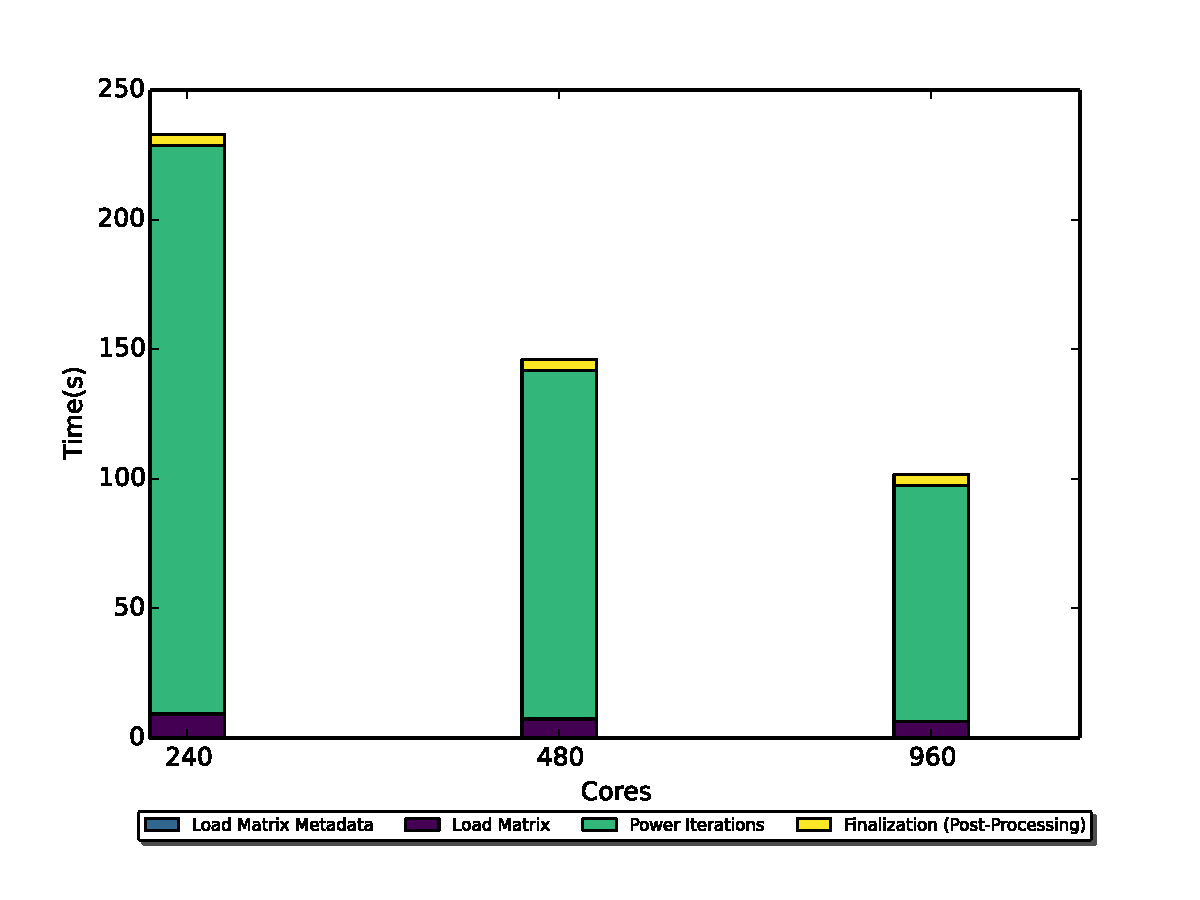
\includegraphics[scale=0.4]{images/CX_Strong_Scaling_New_Colors_Axes_Rank_32_Partitions_default.pdf}
    \end{centering}
    \caption{ Strong scaling for the 4 phases of CX on an XC40 for 100GB dataset at $k=32$ and default partitioning as concurrency is increased.} 
    \label{fig:xc40scaling}
    \end{figure} 

Figure~\ref{fig:xc40scaling} shows how the distributed Spark portion of our code scales as we add additional processors.  We considered 240, 480, and 960 cores.  An additional doubling (to 1920 cores) would be ineffective as there are only 1654 partitions, so many cores would remain unused.  In addition, with fewer partitions per core there are fewer opportunities for load balancing and speculative reexecution of slow tasks.

When we go from 240 to 480 cores, we achieve a speedup of approximately 1.6x from doubling the cores: 233 seconds versus 146 seconds.  However, as the number of partitions per core drops below two, and the amount of computation-per-core relative to communication overhead drops, the scaling slows down (as expected).  This results in a lower speedup of approximately 1.4x (146 seconds versus 102 seconds) when we again double the core count to 960.

  \subsection{CX Performance across Multiple Platforms}
  \label{sect:h2h}
    
    \begin{figure} [h!btp]
    \begin{centering}
    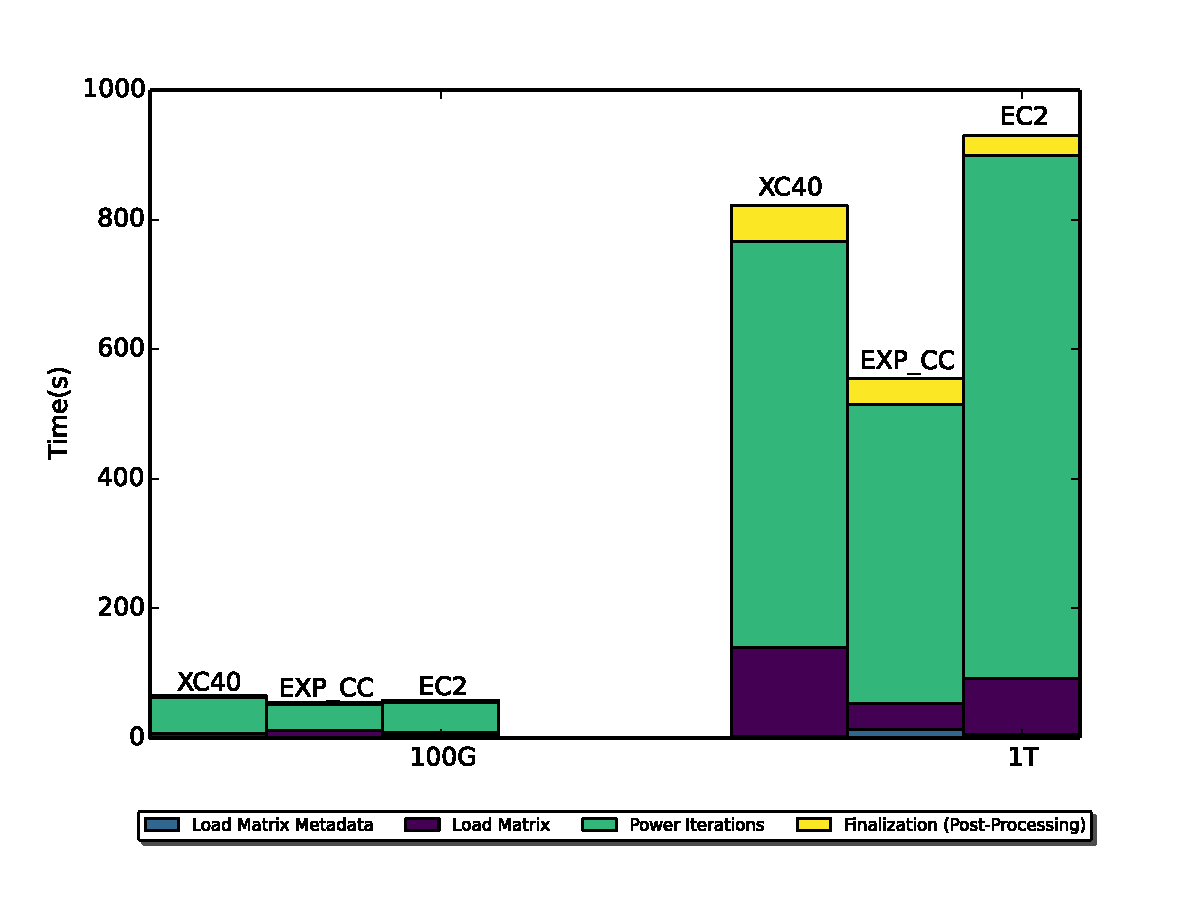
\includegraphics[scale=0.4]{images/CX_Size_Scaling_New_Colors_Axes_Rank_16_Partitions_default.pdf}
    \end{centering}
    \caption{ Run times for the various stages of computation for CX for two different dataset sizes for the three platforms using $k=16$ and default partitioning for the given platform} 
    \label{fig:h2hrank16} 
    \end{figure}

    
      \begin{figure} [H]
    \begin{centering}
    \includegraphics[scale=0.4]{images/CX_Size_Scaling_Rank_32_Partitions_default.pdf}
    \end{centering}
    \caption{ Run times for the various stages of computation for CX for two different dataset sizes for the three platforms using $k=32$ and default partitioning for the given platform}
    \label{fig:h2hrank32} 
    \end{figure}
    
    \begin{table*}
    \begin{center}
    \begin{tabular}{| l | c | c | c | c | c | c | c |}
    \toprule
    \textbf{Platform} & \textbf{Rank} & \textbf{Total} & \textbf{Load} & \textbf{Time Per} & \textbf{Average} & \textbf{Average} & \textbf{Average} \\
                               & & \textbf{Runtime} & \textbf{Time} & \textbf{Iteration} & \textbf{Local} & \textbf{Aggregation} & \textbf{Network} \\
                               & & & & & \textbf{Task} & \textbf{Task} & \textbf{Wait} \\
    \midrule
    Amazon EC2 \texttt{r3.8xlarge} & 16 & 24.0 min & 1.53 min & 2.69 min & 4.4 sec & 27.1 sec & 21.7 sec \\
    \midrule
    Cray XC40 & 16 & 23.1 min& 2.32 min & 2.09 min &  3.5 sec & 6.8 sec & 1.1 sec \\
    \midrule
    Experimental Cray cluster & 16 & 15.2 min & 0.88 min & 1.54 min &  2.8 sec & 9.9 sec & 2.7 sec \\
    \midrule
    Amazon EC2 \texttt{r3.8xlarge} & 32 & 52.6 min& 1.57 min & 5.42 min &  8.7 sec & 60.1 sec & 48.7 sec \\
    \midrule
    Cray XC40 & 32 & 41.2 min & 2.28 min & 4.01 min &  7.5 sec & 25.0 sec & 15.4 sec \\
    \midrule
   Experimental Cray cluster & 32 & 35.8 min & 0.81 min & 3.82 min &  6.8 sec & 27.9 sec & 15.5 sec \\
   \bottomrule
    \end{tabular}
    \end{center}
    \caption{Total runtime for the 1 TB dataset, broken down into load time and per-iteration time. The per-iteration time is further broken down into the average time for each task of the local stage and each task of the aggregation stage.  We also show the average amount of time spent waiting for a network fetch, to illustrate the impact of the interconnect.}
    \label{tab:h2hres1TB}
    \end{table*}
    
Table~\ref{tab:h2hres1TB} shows the total runtime of CX for the 1 TB dataset on our three platforms.  The distributed Spark portion of the computation is also depicted visually in Figures~\ref{fig:h2hrank16} ($k=16$) and~\ref{fig:h2hrank32} ($k=32$).  All three platforms were able to successfully process the 1 TB dataset at $k=16$ in under 25 minutes.  As the table and figures illustrate, most of the variation between the platforms occurred during the \texttt{MultiplyGramian} iterations.  Table~\ref{tab:hwspecs} shows the specifications of the three platforms. In this section, we explore how these difference relate to the performance of the matrix iterations.

Spark divides each iteration into two stages.  The first \emph{local} stage computes each row's contribution, sums the local results (the rows computed by the same worker node), and records these locally-aggregated results.  The second \emph{aggregation} stage combines all of the workers' locally-aggregated results using a tree-structured reduction.  Most of the variation between platforms occurs during the aggregation phase, where data from remote worker nodes is fetched and combined.  In Spark, all inter-node data exchange occurs via \emph{shuffle operations}.  In a shuffle, workers with data to send write the data to their local scratch space.  Once all data has been written, workers with data to retrieve from remote nodes request that data from the sender's block manager, which in turns retrieves if from the senders local scratch space, and sends it over the interconnect to the receiving node.

Examining our three platforms (Table~\ref{tab:hwspecs}), we notice two key hardware differences that impact shuffle operations:
\begin{itemize}
\item First, both the EC2 nodes and the experimental Cray cluster nodes have fast SSD storage local to the compute nodes that they can use to store Spark's shuffle data.  
The Cray{\textsuperscript{\tiny\textregistered}}~XC40{\textsuperscript{\tiny\texttrademark}} system's~\cite{alverson2012cray,craycascadesc12} nodes, on the other hand, have no local persistent storage devices.  Thus we must emulate local storage with a remote Lustre filesystem.  The impacts of this can be somewhat mitigated, however, by leaving sufficient memory to store some of the data in a local RAM disk, and/or to locally cache some of the remote writes to Lustre.\footnote{This is an ideal usage of caching, since Spark assumes the scratch space is only locally accessible; thus we are guaranteed that the only node that reads a scratch file will be the same node that wrote it.}
\item Second, the Cray XC40 and the experimental Cray cluster both communicate over the HPC-optimized Cray Aries 
interconnect~\cite{alverson2012cray,craycascadesc12}, while the EC2 nodes use 10 Gigabit Ethernet.
\end{itemize}  

   \begin{figure} [H]
    \begin{centering}
    \includegraphics[scale=0.4]{images/boxplot_read_write_task_new_Rank_16_1T_default_partitions.pdf}
    \end{centering}
    \caption{A box and whisker plot of the distribution of local (write) and aggregation (read) task times on our three platforms for the 1TB dataset with $k=16$.  The boxes represent the 25th through 75th percentiles, and the lines in the middle of the boxes represent the medians.  The whiskers are set at 1.5 box widths outside the boxes, and the crosses are outliers (results outside the whiskers).  Note that each iteration has 4800 write tasks and just 68 read tasks.}
    \label{fig:rwtaskdist} 
    \end{figure}

We can see the impact of differing interconnect capabilities in the Average Network Wait column in Table~\ref{tab:h2hres1TB}.   These lower average network wait times explain why the two Cray platforms outperform the EC2 instance (with the experimental cluster achieving a speedup of roughly 1.5x over EC2).  

The XC40 is still slightly slower than the experimental Cray cluster, however, in particular at $k=16$.
Part of this difference is due to the slower matrix load phase on the XC40.  On EC2 and the experimental
Cray cluster, the input matrix is stored in SSDs on the nodes running the Spark executors.  Spark is 
aware of the location of the HDFS blocks, and attempts to schedule tasks on the same nodes as their 
input.  The XC40, however, lacks SSDs on its compute nodes, so the input matrix is instead stored on a 
parallel Lustre file system.  The increased IO latency slows the input tasks. The rest of the difference in 
performance can be understood by looking at the distribution of local (write) task times in the box and 
whiskers plot in Figure~\ref{fig:rwtaskdist}.  The local/write tasks are much more numerous than the 
aggregation/read tasks (4800 vs 68 per iteration), thus they have a more significant impact on 
performance. We see that the XC40 write tasks had a similar median time to the experimental cluster's 
write tasks, but a much wider distribution.  The large tail of slower "straggler" tasks is the result of some shuffle data going to the remote Lustre file system rather than being cached locally. We enabled Spark's optional speculative re-execution (\texttt{spark.speculation}) for the XC40 runs, and saw that some of these tasks were successfully speculatively executed on alternate nodes with more available OS cache, and in some case finished earlier.  This eliminated many of the straggler tasks and brought our performance closer to the experimental Cray cluster, but still did not match it (the results in Figures~\ref{fig:h2hrank16} and~\ref{fig:h2hrank32} and Table~\ref{tab:h2hres1TB} include this configuration optimization).  We discuss future directions for improving the performance on Spark on HPC systems in Section~\ref{sect:lessons}.


  
%  \subsection{Timing and Accuracy comparison of RSVD, CX, and truncated SVD}

% Because the RSVD allows us to explicitly control its accuracy by tuning the number of iterations $q$,
% the reconstruction error of the low-rank approximation obtained from the RSVD
% algorithm is expected to be somewhat lower than that of truncated SVD
% approximation. Similarly, CX decompositions have the advantage of
% interpretability, but come at the cost of an increased number of operations on
% top of the RSVD and an additional loss in approximation accuracy. 

%  In Figures~\ref{fig:timing-accuracy-8} and~\ref{fig:timing-accuracy-16}, we observe the timing vs accuracy tradeoffs of the RSVD and CX algorithms
%  as applied to the 100G MSI dataset for two settings of the rank parameter, $k=8$ and $k=16$. The exact SVD was computed in this case using the
%  Spark bindings of the popular ARPACK eigenproblem library~\cite{ArpackUserGuide}. The RSVD algorithm used two power iterations, and we used the output of the RSVD algorithm to generate
%  both the column CX decomposition defined in Algorithm~\ref{alg:cx} and a related `row CX' decomposition that comes from applying Algorithm~\ref{alg:cx}
%  to $A^T.$ As explained in more detail in the next section, both of these CX decompositions are of interest, as they identify important pixels and ions.
%
%  For both rank parameters, we observe the behavior predicted by the theory for the RSVD decomposition: the approximation error is only slightly greater than that of the 
%  truncated SVD approximation. We also observe that there is only a slight speed advantage to using the RSVD; this is likely attributable to the fact that the input matrix
%  is truly low-rank (more than 70\% of the Frobenius norm of the matrix is already captured by the rank-8 decomposition), so the iterative ARPACK SVD algorithm converges 
%  quite fast.
%
%  The CX decompositions require significantly more time to compute than the truncated SVD and RSVD decompositions. This is due to the need to compute the projection of $A$ onto
%  the columns $C$ after $C$ is constructed according to Algorithm~\ref{alg:cx}. We also note that for the MSI dataset, row-based CX decompositions are more 
%  accurate and less expensive to construct than column-based CX decompositions. 
%
%  \begin{figure}[h!btp]
%    \begin{centering}
%      \includegraphics[scale=0.4]{images/timing-accuracy-8}
%      \end{centering}
%      \caption{The Frobenius norm approximation errors and timings for three runs of the RSVD and CX approximations relative to those of the truncated SVD for a target rank of $8$ on the 100G MSI dataset.}
%    \label{fig:timing-accuracy-8}
%  \end{figure}
%
%  \begin{figure}[h!btp]
%    \begin{centering}
%      \includegraphics[scale=0.4]{images/timing-accuracy-16}
%      \end{centering}
%      \caption{The Frobenius norm approximation errors and timings for three runs of the RSVD and CX approximations relative to those of the truncated SVD for a target rank of $16$ on the 100G MSI dataset.}
%    \label{fig:timing-accuracy-16}
%  \end{figure}

  \subsection{Science Results}
  \subsubsection{CX}
  
  \begin{figure}[h!bt]
    \centering
    \includegraphics[width=.9\columnwidth]{images/cx_ions.pdf}
      \caption{Normalized leverage scores (sampling probabilities) for $m/z$ marginalized over $\tau$.
        Three narrow regions of $m/z$ account for $59.3\%$ of the total probability mass.}
      \label{fig:cx_ions}
  \end{figure} 

  Here, we examine the results of the CX decomposition of the MSI dataset.
  The rows and columns of our data matrix $A$ correspond to pixels and $(\tau, m/z)$ values of ions, respectively. 
  We compute the CX decompositions of both $A$ and $A^T$ in order to identify important ions in addition to important pixels.
   
  In Figure~\ref{fig:cx_ions}, we present the distribution of the normalized
  ion leverage scores marginalized over $\tau$. That is, each score corresponds
  to an ion with $m/z$ value shown in the $x$-axis. Leverage scores of ions in
  three narrow regions have significantly larger magnitude than the rest. This
  indicates that these ions are more informative and should be kept as basis
  for reconstruction.  Encouragingly, several other ions with significant
  leverage scores are chemically related to the ions with highest leverage
  scores.  For example, the ion with an $m/z$ value of 453.0983 has the second
  highest leverage score among the CX results.  Also identified as having
  significant leverage scores are ions at $m/z$ values of 439.0819, 423.0832,
  and 471.1276, which correspond to neutral losses of $\rm{CH_2}$,
  $\rm{CH_2O}$, and a neutral ``gain'' of $\rm{H_2O}$ from the 453.0983 ion.
  These relationships indicate that this set of ions, all identified by CX as
  having significant leverage scores, are chemically related.  That fact
  indicates that these ions may share a common biological origin, despite
  having distinct spatial distributions in the plant tissue sample.

  \subsection{Improving Spark on HPC Systems}
  \label{sect:lessons}
  
  The differences in performance between the Cray{\textsuperscript{\tiny\textregistered}}~XC40{\textsuperscript{\tiny\texttrademark}} system~\cite{alverson2012cray,craycascadesc12} and the experimental Cray cluster point to optimizations to Spark that could improve its performance on HPC-style architectures.  The two platforms have very similar configurations, with the primary difference being the lack of local persistent storage on the XC40 nodes.  As described in Section~\ref{sect:h2h}, this forces some of Spark's local scratch space to be allocated on the remote Lustre file system, rather than in local storage.  To mitigate this, and keep more of the scratch data local, we propose the following future work:
\begin{itemize}
\item Spark is currently inefficient in cleaning up its local scratch space.  In particular, shuffle data is not immediately cleaned up after a shuffle completes.  This makes fault recovery more efficient, but results in higher storage requirements for scratch space.  If clean up was more efficient, it would be more feasible to fit all of the scratch data in a local RAM disk and not rely on Lustre at all.
\item Spark does not currently allow you to configure primary and backup scratch directories.  Instead you list all scratch directories in a single list, and it distributes data in a round round fashion between them as long as space is available.  You can bias it towards one storage device (e.g., RAM disk vs. Lustre) by listing multiple directories on the preferred device.  Ideally, though, we would like to use a RAM disk (or other local storage) exclusively unless and until it fills, and only switch to Lustre directories if necessary.
\item Spark does not allow you to specify that a scratch directory is globally accessible.  Thus non-cached data is stored to the remote Lustre directory by the sender, and then later retrieved by the sender and sent to the receiver.  This wastes a step, since the receiver could easily fetch the data directly from Lustre (or any other global file system).
\item Alternatively, a push model of communication (as opposed to the current pull model) might be possible - however this would have implications for reliability and handling of very large data sets.\footnote{Storing the shuffle data to a large persistent block storage device, and only sending it as needed, allows Spark to easily shuffle more data than could fit in the remote buffers.  In a push-based model, extra logic and synchronization would be necessary to ensure that the remote buffers do not overflow.}
\end{itemize}



\section{Conclusions}
\label{sec:conclusion}

Matrix factorizations are an important class of linear algebra computations
with broad applications in Big Data analytics. In this work, we have
successfully developed highly optimized versions of the CX algorithm, both on a
single node, as well as distributed multi-node implementations. We utilize
Spark as a contemporary data analytics framework for developing and deploying
the CX algorithm, and successfully demonstrate the implementaton scaling up to
960 cores. We evaluate our parallel implementation on HPC and EC2 class
hardware; we find that faster interconnects enable the numerically intensive
computations to run more efficiently on HPC systems. Finally, this scalable
implementation was used to analyze a large scale, TB-sized mass-spec imaging
dataset; the resulting ion and spatial patterns obtained from the analysis are
providing biologist with novel insights on complex molecular mechanisms in
cells. 


\section{Dummy Citation}
Dummy citation for Bib\TeX:
\LaTeX\cite{Lamport:LaTeX}


%
% The following two commands are all you need in the
% initial runs of your .tex file to
% produce the bibliography for the citations in your paper.
\bibliographystyle{abbrv}
\bibliography{heromsi}

\subsection{References}
Generated by bibtex from your ~.bib file.  Run latex,
then bibtex, then latex twice (to resolve references)
to create the ~.bbl file.  Insert that ~.bbl file into
the .tex source file and comment out
the command \texttt{{\char'134}thebibliography}.

\balancecolumns
% That's all folks!
\end{document}
